%% ============================================================
%%  Springer Nature / Nature-family journal template
%%  Class file required: sn-jnl.cls
%%  Download: https://www.springernature.com/gp/authors/campaigns/latex-author-support
%%  Target journal: Nature Machine Intelligence  (primary submission target)
%%
%%  This is the single entry file for the paper. Build: ./run.sh
%%  (pdflatex → bibtex → pdflatex × 2  →  main.pdf)
%%  NMI reframing toggle \ifNMIframing (default on); see README.md §4 / §8.
%% ============================================================

\documentclass[
    %% --- journal style options (pick one) ---
    % iicol,          % two-column (IEEE-like preview; final layout set by editors)
    Numbered,         % numbered references  ← Nature style
]{sn-jnl}

%% ---- Springer Nature bibliography style -----------------
%% sn-nature          : Nature-family superscript numeric
%% sn-mathphys-num    : numbered, brackets
%% sn-aps             : APS style
\usepackage[numbers,sort&compress]{natbib}

%% ---- Standard packages ----------------------------------
\usepackage{amsmath,amssymb,amsfonts}
\usepackage{graphicx}
\usepackage{xcolor}
\usepackage{hyperref}
\hypersetup{colorlinks=true, linkcolor=blue, citecolor=blue, urlcolor=blue,
bookmarks=true, bookmarksopen=true,
pdftitle={Situation engineering for reliable evidence use in artificial intelligence},
pdfauthor={Geunsik Lim},
pdfsubject={Situation engineering, evidence applicability and reliable AI},
pdfkeywords={situation engineering, evidence applicability, reliable AI, temporal reasoning, hallucination}}
\usepackage{booktabs}
\usepackage{tabularx}
\usepackage{makecell}
\usepackage{algorithm}
\usepackage[noend]{algpseudocode}
\usepackage{pifont}
\usepackage{soul}
\usepackage{listings}
\usepackage{float}
\usepackage{placeins}
\usepackage{ifthen}
\usepackage{diagbox}

%% ---- Experiment-reporting helpers (kept from original) ---
\newcommand{\ntrials}{5}
\newcommand{\ci}{95\%~CI}
\newcommand{\hwsetup}{2~$\times$~NVIDIA~A100~(80\,GB), 512\,GB DRAM, NVMe Gen4}
\newcommand{\swsetup}{PyTorch~2.4, CUDA~12.2, vLLM~\cite{kwon2023pagedattention}~0.5.3}
\newcommand{\capinfo}{\emph{Means across $n=\ntrials$ runs (\ci). HW: \hwsetup; SW: \swsetup.}}

%% ---- ORCID icon (optional) ------------------------------
\usepackage{scalerel}
\usepackage{tikz}
\usetikzlibrary{svg.path,positioning,arrows.meta,fit}
\definecolor{orcidlogocol}{HTML}{A6CE39}
\tikzset{
  orcidlogo/.pic={
    \fill[orcidlogocol] svg{M256,128c0,70.7-57.3,128-128,128C57.3,256,0,198.7,0,128C0,57.3,57.3,0,128,0C198.7,0,256,57.3,256,128z};
    \fill[white] svg{M86.3,186.2H70.9V79.1h15.4v48.4V186.2z}
                 svg{M108.9,79.1h41.6c39.6,0,57,28.3,57,53.6c0,27.5-21.5,53.6-56.8,53.6h-41.8V79.1z M124.3,172.4h24.5c34.9,0,42.9-26.5,42.9-39.7c0-21.5-13.7-39.7-43.7-39.7h-23.7V172.4z}
                 svg{M88.7,56.8c0,5.5-4.5,10.1-10.1,10.1c-5.6,0-10.1-4.6-10.1-10.1c0-5.6,4.5-10.1,10.1-10.1C84.2,46.7,88.7,51.3,88.7,56.8z};
  }
}
\newcommand\orcidicon[1]{\href{https://orcid.org/#1}{\mbox{\scalerel*{
\begin{tikzpicture}[yscale=-1,transform shape]
\pic{orcidlogo};
\end{tikzpicture}
}{|}}}}

%% ---- Anonymity switch (1 = named, 0 = anonymous) --------
\newcommand{\anonymous}{0}

%% =============================================================
%% NMI framing toggle
%% -------------------------------------------------------------
%% 1차 투고 대상 = Nature Machine Intelligence.
%% \NMIframingtrue  → NMI용 재프레이밍(초록·서론) 사용 (기본값).
%% \NMIframingfalse → 기존 NCS/Nature 서사로 복귀.
%% 근거·전략: README.md §8·§9 참조.
\newif\ifNMIframing
\NMIframingtrue
%% =============================================================

%% =============================================================
%% Reference URL toggle
%% -------------------------------------------------------------
%% 리뷰(열람)용 사본에는 각 참고문헌의 URL을 출력한다 (기본값).
%% \RefURLstrue  → 참고문헌마다 URL을 파란색으로 출력 (사전 열람용).
%% \RefURLsfalse → 저널 제출용: URL 출력 안 함.
%% URL 색은 전역 hypersetup과 무관하게 항상 파란색으로 고정한다.
\newif\ifRefURLs
\RefURLsfalse
\newcommand{\refurl}[1]{\ifRefURLs\ {\color{blue}\url{#1}}\fi}
%% =============================================================

%% =============================================================
%% E5 (multi-model intervention) toggle
%% -------------------------------------------------------------
%% E5 결과(실제 frontier/open 모델 응답)가 준비되면 아래를 true로.
%% \E5readytrue  → Results에 E5 절과 tab:e5-multimodel 표를 포함.
%% \E5readyfalse → 기본값(제출 청결): E5 절 미포함.
%% 실행 경로: OPENROUTER_API_KEY 설정 후 `python code/run_e5.py`가
%% paper/results/multimodel_summary.csv → section/tables/e5_multimodel_table.tex
%% 를 자동 생성한다(실데이터 없으면 PENDING placeholder). 자세한 내용은
%% code/experiment_manifest.e5.json 참조.
\newif\ifE5ready
\E5readyfalse
%% =============================================================

%% =============================================================
%% NMI REVIEWER ANTICIPATION MAP  (non-printing; address before submission)
%% -------------------------------------------------------------
%% These are LaTeX comments only and never appear in the compiled PDF.
%% They record the concerns a Nature Machine Intelligence referee is most
%% likely to raise, each with a severity, the current status, the concrete
%% revision action, and the section that must carry it. Work top-down: the
%% two CRITICAL items decide accept/reject; the rest strengthen the case.
%%
%% [R1] CRITICAL — Headline oracle result is analytic, not empirical.
%%   Concern: SCQA 100.0% vs the 85.7% control is a deterministic
%%     consequence of the construction (equal category weights => 6/7 =
%%     85.7%). A tautology cannot support a claim of advance.
%%   Status: acknowledged in Results, but referees still weight it heavily.
%%   Action: present oracle numbers strictly as regression-test coverage,
%%     never as an effect size; lead Results with the causal ablations and
%%     the predicted-state sensing bottleneck, not the 100/85.7 gap.
%%   Section: 025_results_ncs.
%%
%% [R2] CRITICAL — No evidence situation engineering helps a real model.
%%   Concern: by the evidence ladder, E5 (matched multi-model intervention)
%%     and E6 (deployment/human) are not done; the paper shows a symbolic
%%     solver passing a symbolic test, not that explicit state helps an LLM.
%%   Status: honestly scoped, but reads as a Perspective, not a Research
%%     Article, at NMI's bar.
%%   Action: complete E5 on real models via code/run_e5.py (gated by
%%     code/audit_e5.py); flip \E5readytrue and report the within-model
%%     situation-vs-baseline contrast. Until then, state E5 as preliminary.
%%   Section: 026_results_e5 (+ abstract, evidence-ladder row).
%%
%% [R3] MAJOR — Benchmark-solver circularity / no natural language.
%%   Concern: diagnostic data are generated from the same schema the solver
%%     consumes; even the 77.9% predicted-state number is a rule sensor on
%%     templated text (time/validity slots score 0% by construction).
%%   Action: add a natural-language evaluation (SituatedQA/FreshQA/TDBench-
%%     derived); state external validity limits explicitly.
%%   Section: 025_results_ncs, Discussion limitations; data/ expansion.
%%
%% [R4] MAJOR — Novelty is largely organisational.
%%   Concern: heavy overlap with cited traditions (situation/event calculus,
%%     belief revision/TMS, POMDP/DST, bitemporal DBs); the new element is a
%%     "systems contract", not a demonstrated new capability.
%%   Action: sharpen the one concrete, testable capability the contract adds
%%     beyond a structured prompt, and show it empirically (ties to R2).
%%   Section: 012_related_work, 015_situation_engineering.
%%
%% [R5] MINOR/MAJOR — Statistical framing.
%%   Concern: 4,200 items overstate independence (shared template families);
%%     confidence values are rule-derived, not calibrated.
%%   Action: cluster/bootstrap CIs over template families for key contrasts;
%%     add selective-risk / risk-coverage curves; avoid over-precise 100.0%.
%%   Section: 025_results_ncs, Methods.
%%
%% REVISION CHECKLIST to reach NMI-accept grade (see paper/E5_COMPLETION_CHECKLIST.md):
%%   (a) >=3 model FAMILIES, matched evidence/token/cost budgets;
%%   (b) natural-language set; (c) strong RAG/structured-prompt baselines;
%%   (d) human inter-annotator agreement (code/annotation_cli.py);
%%   (e) clustered uncertainty + selective risk; (f) cost/latency accounting;
%%   (g) archival DOI + licence before acceptance.
%% Referee's current call: reject-and-resubmit; the above converts it.
%% =============================================================

%% =============================================================
%% PER-SECTION REVISION NOTES  (non-printing; consolidated here on purpose)
%% -------------------------------------------------------------
%% Every actionable edit is kept in this file rather than scattered as inline
%% comments across section/*.tex, so main.tex is the single control surface for
%% the reviewer response. Tags [R1]-[R5] refer to the map above. Do the edits
%% inside the named \input files; this list is the checklist.
%%
%% 001_title.tex
%%   [R4] Keep the title's claim within what is demonstrated ("reliable
%%        evidence use", not "solved situation understanding").
%%
%% 006_abstract_nmi.tex
%%   [R1] Do not lead with 100.0%; call oracle numbers regression coverage.
%%   [R2] The abstract pre-announces "matched natural-text and multi-model
%%        tests" -- until \E5readytrue, phrase E5 as a pre-specified/pending
%%        test, not an achieved result.
%%
%% 010_introduction_nmi.tex
%%   [R4] State plainly the one concrete capability the situation contract
%%        adds beyond a structured prompt, and promise its empirical test (R2).
%%   [R2] Keep contribution claims bounded to E1-E4 as established.
%%
%% 012_related_work.tex
%%   [R4] Add an explicit head-to-head contrast with the closest prior work
%%        (situation/event calculus, dialogue-state tracking); operationalise
%%        the vague Table cells ("limited"/"partial") with a concrete criterion.
%%
%% 015_situation_engineering.tex
%%   [R4] Turn the contract (C_t,M_t,O_t,H_t)->(S_t,U_t,P_t) into at least one
%%        falsifiable prediction that a non-situational baseline should fail.
%%
%% 025_results_ncs.tex
%%   [R1] Frame 100.0% vs 85.7% as regression-test coverage; lead with the
%%        causal ablations and the predicted-state sensing bottleneck.
%%   [R3] State benchmark-solver circularity up front; explain the 0% time/
%%        validity slots as a construction artifact, not a language finding.
%%   [R5] Report clustered/bootstrap CIs over template families for the key
%%        contrasts; add a selective-risk / risk-coverage view.
%%
%% 026_results_e5.tex  (enabled by \E5readytrue)
%%   [R2] Populate from code/run_e5.py once code/audit_e5.py prints
%%        "E5 INTEGRITY GATE: PASS"; report the within-model
%%        situation-vs-baseline delta and label the scope honestly
%%        (provider family, models, N, conditions, decoding).
%%
%% 060_discussion.tex
%%   [R3] Make external-validity limits explicit (synthetic templates; single
%%        family in any preliminary E5).
%%   [R2] Say precisely what E5 does and does not license.
%%
%% 070_methods.tex
%%   [R5] Describe the clustered/bootstrap CI procedure and the template-family
%%        unit of analysis; either report the multi-model adapter results or
%%        move its description to Discussion so Methods matches the claims.
%% =============================================================

%% =============================================================
\begin{document}
%% =============================================================

%% ---- Title -------------------------------------------------
%% Title for Nature Machine Intelligence
%% NOTE (co-author revision): the title now foregrounds the demonstrated
%% contribution -- separating evidence applicability from availability -- rather
%% than an unproven "reliability" outcome, to match the bounded, null-to-negative
%% E5 result. Revert to the previous wording only if the confirmatory
%% multi-family experiment establishes a reliability improvement.
\title{Situation engineering: separating evidence applicability from availability in AI systems}


%% ---- Authors & Affiliations --------------------------------
%% ============================================================
%%  Author & Affiliation block — sn-jnl format
%%  sn-jnl uses \author / \affil macros (not IEEEauthorblock)
%% ============================================================

\ifnum\anonymous=1
  %% --- Blind review version ---
  \author*{\fnm{Anonymous} \sur{Author(s)}}
  \affil*{\orgname{Anonymous Institution}}
\else
  %% --- Camera-ready version ---
  \author*[1]{\fnm{Geunsik} \sur{Lim}\orcidicon{0000-0003-1845-7132}}
  \email{leemgs@g.skku.edu}

  \affil[1]{
    \orgdiv{College of Information and Communication Engineering},
    \orgname{Sungkyunkwan University},
    \orgaddress{
      \city{Suwon},
      \country{South Korea}
    }
  }
\fi

%% \maketitle is issued in main.tex AFTER the abstract is defined:
%% sn-jnl renders \abstract{...} inside \maketitle, so calling it here
%% would silently drop the abstract from the PDF.


%% ---- Abstract & Keywords -----------------------------------
\ifNMIframing
  \abstract{%
Artificial-intelligence systems can retrieve a well-supported fact yet apply it
to the wrong time, scope, epistemic state or possible world. We call this
failure \emph{situation blindness} and define \emph{situation engineering} as
constructing the query-relative state that governs evidence applicability. We
introduce a state interface, Situation-Catching Question Answering, and
SituationCatch-Bench, a 4,200-item diagnostic spanning temporal change, missing
premises, source conflict, modality, scope, observer knowledge and counterfactual
worlds. A deterministic implementation satisfies every invariant under
oracle states; accuracy falls to 77.9\% under text-inferred states and 35.1\%
after corruption, and matched ablations produce category-specific failures.
These results establish an executable diagnostic, not language-model
superiority. In a preliminary single-family test (three Gemini models,
$n=210$), explicit situation prompting does not beat matched structured
prompting and trails focused retrieval, leading only on temporal and observer
items; these category comparisons are exploratory. This
bounded result is consistent with applicability \emph{sensing}, not a prompt
slot, being the bottleneck.
}

\keywords{large language models, situation engineering, evidence applicability, situation awareness, hallucination, trustworthy artificial intelligence, temporal reasoning, question answering, agent systems}
      % NMI framing (Nature syntax)
\else
  \input{./section/006_abstract_nature.tex}   % original NCS/Nature abstract
\fi

%% sn-jnl emits the abstract inside \maketitle, so it must come after
%% the \abstract{...} definition above.
\maketitle

%% ---- Main text (NCS structure: Intro → Results → Discussion) ---
\ifNMIframing
  \pdfbookmark[1]{Introduction}{bookmark-introduction}
  \label{sec:introduction}

Large language models (LLMs) increasingly answer questions by combining
parametric knowledge with retrieved documents, tools, memory and long
conversational histories. These mechanisms improve evidence coverage, but they
do not guarantee that a system identifies the \emph{situation} in which a fact
is valid. A model may read that a person was appointed and later resigned, yet
still name that person as the current office holder. It may turn a proposal
into a decision, extend a local policy to an entire organization, answer from
information unavailable to the queried observer, or collapse a hypothetical
scenario into the real world. In each case the decisive evidence can already be
present. The failure is not simply missing knowledge; it is incorrect evidence
applicability.

We define \emph{situation blindness} as producing an answer or action that is
supported by at least one available claim but inconsistent with the time, scope,
modality, observer knowledge or possible world required by the query. This
category matters because conventional factuality checks can mark the supporting
claim as true while missing that it is true in the wrong situation. Natural
question-answering resources already show that a material subset of ordinary
questions depends on extra-linguistic time or place, and that updated evidence
does not eliminate the resulting performance loss~\cite{zhang2021situatedqa,
vu2023freshqa,meem2024pat,chen2021timeqa,chen2025chronoqa}.

Retrieval-augmented generation supplies external evidence~\cite{lewis2020rag};
self-reflective and tool-using systems add critique and action
~\cite{asai2024selfrag,yao2023react,schick2023toolformer}; context engineering
organizes the inference-time information payload~\cite{mei2025context}; and
agent harnesses mediate tools, memory, permissions, verification and feedback
~\cite{zhong2026harness,lin2026ahe}. These layers are necessary, but none
requires an explicit answer to a separate question: \emph{which interpretation
of the available evidence governs this interaction now?}

We call the corresponding discipline \emph{situation engineering}: the
systematic design of representations, sensing interfaces, update rules,
validation procedures and response policies that establish the active
query-relative world state before an AI system commits to an answer or action.
For a query $q$ and evidence $E$, a minimal state is
\begin{equation}
S(q,E)=\{\mathcal{A},\mathcal{V},\mathcal{T},\mathcal{P},\mathcal{M},
\mathcal{K},\mathcal{W},\mathcal{U}\},
\end{equation}
where the variables denote actors, events, valid time, scope, modality and
source status, observer-specific knowledge, possible world and unresolved
answer-critical information. A policy then selects
\begin{equation}
\pi(S)\in\{\textsc{Answer},\textsc{Clarify},\textsc{Retrieve},
\textsc{Abstain},\textsc{Act}\}.
\end{equation}
This decomposition separates evidence availability from evidence applicability.

We organize the study around three questions.
\textbf{RQ1 (representation):} can failures involving time, scope, modality,
source status, observer knowledge, possible world and missing information be
expressed through one inspectable applicability interface?
\textbf{RQ2 (localization):} when that interface fails, can matched controls
separate state-sensing errors from update, validation and response-policy
errors?
\textbf{RQ3 (transfer):} does exposing the interface to current LLMs improve
answers beyond equally informed structured, retrieval and tool-using
baselines? RQ1 and RQ2 are evaluated as controlled software and mechanistic
claims. RQ3 is a deliberately bounded pilot and remains open as a general
empirical claim.

This question structure yields four contributions with different evidential
status. First, we operationalize \emph{situation blindness}: correctness
requires both evidential support and query-relative applicability. Second, we
specify a systems contract connecting sensing, provenance-linked state,
validation and answer/retrieve/clarify/abstain/action policy, while leaving the
choice of logical, probabilistic or neural implementation open. Third, we
release SCQA and SituationCatch-Bench as mechanism-level diagnostics: matched
state conditions and component ablations test whether each declared variable
has its predicted behavioural consequence. Fourth, we contribute a negative
and therefore informative boundary result. In an audited three-model
Gemini-family pilot, an explicit situation prompt is null-to-negative against a
matched structured prompt and trails focused retrieval overall. This prevents
the framework contribution from being conflated with prompt superiority and
pre-specifies the natural-text, multi-family and human-agreement evidence
needed to test transfer.
         % NMI-reframed introduction
\else
  \input{section/010_introduction}             % original introduction
\fi
\pdfbookmark[1]{Related Work}{bookmark-related}
\section*{Related conceptual foundations}

Situation engineering draws on several mature traditions but is not identical
to any one of them. Situation semantics treats meaning relative to partial
situations~\cite{barwise1983situations}. Situation and event calculi formalize
how actions change fluents over time~\cite{mccarthy1969problems,
kowalski1986event,reiter2001knowledge}. Temporal reasoning provides interval
relations and validity semantics~\cite{allen1983interval}. Belief revision and
truth-maintenance research asks how an agent should update inconsistent
commitments~\cite{alchourron1985logic,doyle1979truth}. POMDPs and dialogue-state
tracking maintain uncertainty over latent states for sequential decisions
~\cite{kaelbling1998pomdp,henderson2014second}. Temporal knowledge graphs and
bitemporal databases record changing facts and distinguish when a fact is valid
from when it is stored~\cite{snodgrass1992temporal}.

The proposed contribution is a systems-level applicability contract for
generative and agentic AI. It requires these representations to connect to
natural-language evidence, provenance, unresolved alternatives and a response
policy that can answer, retrieve, clarify, abstain or act. Thus the novelty is
not a new universal logic. It is the explicit decomposition of modern AI
reliability into (i) sensing a situation from heterogeneous evidence, (ii)
maintaining a provenance-linked state, (iii) validating applicability and
(iv) propagating unresolved state into behaviour. This framing allows existing
logical, probabilistic and neural methods to be compared through a common set of
interfaces and failure measurements.

A key distinction is that these traditions vary in whether they jointly expose
time, observer, possible world, uncertainty, provenance and an answer-or-action
gate; the proposed interface requires all of them to be reportable without
claiming that their underlying formalisms are new. The comparison criterion is
therefore not terminological coverage but \emph{diagnostic accountability}:
whether a wrong output can be localized to sensing, update, validation, policy
or generation and tested by holding the other stages fixed.


Dynamic epistemic logic and common-ground modelling formalize belief-changing
information and mutually recognized conversational commitments
~\cite{vanbenthem1996dynamic,stalnaker2002common}. Theory-of-mind models, world
models and active perception further address attributed beliefs, latent
environment state and information acquisition. These traditions reinforce rather
than eliminate the need for careful attribution: situation engineering does not
claim their theoretical results as new. Its proposed novelty is the systems
contract that exposes their state variables to provenance-aware
answer/retrieve/clarify/abstain gates in contemporary generative systems.

\pdfbookmark[1]{Situation Engineering Framework}{bookmark-framework}
\section*{Situation Engineering framework}

Prompt engineering specifies a task; context and retrieval engineering select
information; memory engineering retains observations; tools expose
capabilities; and harness engineering controls execution. Situation engineering
addresses a narrower semantic question: which available claims apply to this
query, observer and world now? It is therefore a proposed interface among
existing components, not a replacement name for them and not an empirically
validated universal layer.

For query $q$, evidence $E$, retained memory $M_t$, tool observations $O_t$ and
harness trace $H_t$, situation construction produces candidate states
$\mathcal{S}_t$ with unresolved variables $U_t$ and provenance $P_t$:
\begin{equation}
(q,E,M_t,O_t,H_t)\rightarrow(\mathcal{S}_t,U_t,P_t).
\end{equation}
Each evidence claim is assigned a query-relative applicability value
\begin{equation}
\mathrm{Apply}(e,q,S_t)\in
\{\mathrm{valid},\mathrm{invalid},\mathrm{unresolved}\}.
\end{equation}
Preserving \emph{unresolved} is essential. A system should retrieve, clarify or
abstain when answer-critical state cannot be established rather than silently
converting uncertainty into a plausible binary judgement.

\begin{figure}[t]
\centering
\resizebox{\linewidth}{!}{\begin{tikzpicture}[
every node/.style={font=\small}, box/.style={draw,rounded corners,align=center,
minimum height=8mm}, arr/.style={-{Latex},thick}]
\node[anchor=west,font=\bfseries] at (0,4.5) {(a) Failure};
\node[box,text width=2.8cm] (appointed) at (3.0,4.5) {appointed at $t_1$};
\node[box,text width=2.8cm] (resigned) at (7.0,4.5) {resigned at $t_2$};
\node[box,text width=3.4cm,fill=red!8] (question) at (11.5,4.5) {Who is current at $t_3$?};
\draw[arr] (appointed)--(resigned); \draw[arr] (resigned)--(question);

\node[anchor=west,font=\bfseries] at (0,3.0) {(b) Retrieval only};
\node[box,text width=3.0cm] (claims) at (3.0,3.0) {relevant claims};
\node[box,text width=3.0cm] (rank) at (7.0,3.0) {rank / concatenate};
\node[box,text width=3.4cm,fill=red!8] (answer) at (11.5,3.0) {supported answer};
\draw[arr] (claims)--(rank); \draw[arr] (rank)--(answer);

\node[anchor=west,font=\bfseries] at (0,1.5) {(c) Situation engineering};
\node[box,text width=3.0cm] (input) at (3.0,1.5) {query, evidence,\\memory, tools};
\node[box,text width=3.0cm] (state) at (7.0,1.5) {sense + update\\provenance-linked state};
\node[box,text width=3.4cm,fill=green!10] (policy) at (11.5,1.5) {validate applicability\\answer / retrieve / clarify / abstain};
\draw[arr] (input)--(state); \draw[arr] (state)--(policy);

\node[anchor=west,font=\bfseries] at (0,0) {(d) Diagnostic axes};
\node[box,text width=11.0cm] at (7.2,0) {time \quad scope \quad modality \quad source conflict \quad observer \quad world \quad unresolved premise};
\end{tikzpicture}}
\caption{From situation blindness to an applicability-aware response.
\textbf{a}, A supported appointment becomes stale after resignation.
\textbf{b}, retrieval and relevance alone do not require resolution of that
transition. \textbf{c}, situation engineering constructs a provenance-linked
state, validates claim applicability and propagates unresolved variables into
response policy. \textbf{d}, SituationCatch-Bench isolates seven corresponding
diagnostic axes.}
\label{fig:engineering-planes}
\end{figure}

\subsection*{Operations and component boundaries}

Six operations define the interface. \emph{Sensing} extracts actors, events,
times, modality, source status, scope, observer knowledge and world identity.
\emph{Assembly} links observations into candidate states. \emph{Updating}
applies supersession, cancellation and belief transitions. \emph{Validation}
checks applicability, conflicts, provenance and missing variables.
\emph{Policy} selects an answer, retrieval, clarification, abstention or action.
\emph{Observability} records the active state and its evidence.

These responsibilities do not absorb neighbouring disciplines. A retriever
still owns ranking and freshness; a memory system owns retention; a tool layer
owns invocation semantics; a harness owns permissions and recovery; and serving
systems own resource efficiency. The proposed situation layer consumes their
outputs and returns applicability decisions and unresolved-state signals.
Likewise, longer context is not sufficient: it may contain an appointment and
a later resignation, a proposal and a final decision, or real and hypothetical
claims simultaneously. Applicability requires resolving their relation rather
than merely retaining both.

\subsection*{SCQA as a bounded control implementation}

Situation-Catching Question Answering (SCQA) instantiates the interface for
seven controlled variables. Its deterministic sensor or supplied gold state
feeds auditable update rules and an answer/clarify/abstain policy. SCQA has no
learned parameters. It is designed to test whether removing a required variable
produces the matching failure signature, not to compete with contemporary
language models.

This scope matters for interpretation. The generated benchmark and solver share
an ontology, making the oracle-state experiment analogous to a protocol
conformance suite. The predicted-state condition introduces sensing error but
still uses generated English. Natural-language generalization, comparison with
strong prompting and retrieval systems, multilingual transfer, human
annotation and deployment efficiency remain untested hypotheses. The released
multi-provider and annotation programs make these studies executable but do not
turn an unexecuted protocol into evidence.

\subsection*{Testable predictions}

The framework yields falsifiable predictions for future matched experiments.
Holding model, evidence and computation budget fixed, an explicit situation
state should improve the categories whose decisive variables are otherwise
implicit. Gains should diminish when a baseline already represents the same
state. Predicted-state errors should decompose into sensing, update, policy and
generation failures. Corrupting one state slot should selectively damage its
matching category. Finally, the benefit must be evaluated jointly with token
use, latency, retrieval calls, monetary cost and unnecessary clarification.
Failure of these predictions would argue against treating situation engineering
as a distinct practical interface.

\pdfbookmark[1]{Results}{bookmark-results}
\section*{Results}

\subsection*{A controlled benchmark isolates seven applicability invariants}

SituationCatch-Bench v0.1 contains 4,200 generated English instances, with 600
instances in each of seven diagnostic categories: temporal state change,
omitted answer-critical premises, source conflict, proposed versus confirmed
events, local versus universal scope, observer-dependent knowledge and real
versus counterfactual worlds. Every item provides a question, shuffled claims,
query time, required state variables, a gold action and, where answerable, a
gold answer. The benchmark is intentionally transparent: each category is a
software-level test of one applicability invariant rather than a claim to
natural linguistic diversity.

\begin{figure}[t]
\centering
\begin{tikzpicture}[node distance=7mm and 7mm, every node/.style={font=\small}]
\node[draw,rounded corners,align=center,minimum width=23mm] (e) {Evidence and\\query};
\node[draw,rounded corners,align=center,right=of e,minimum width=25mm] (s) {Situation\\sensing};
\node[draw,rounded corners,align=center,right=of s,minimum width=25mm] (u) {State update\\and validation};
\node[draw,rounded corners,align=center,right=of u,minimum width=25mm] (p) {Response\\policy};
\node[draw,rounded corners,align=center,below=of p,minimum width=26mm] (o) {Answer / retrieve /\\clarify / abstain};
\draw[-{Latex}] (e)--(s); \draw[-{Latex}] (s)--(u); \draw[-{Latex}] (u)--(p); \draw[-{Latex}] (p)--(o);
\end{tikzpicture}
\caption{Evaluation decomposition. The present experiment supplies oracle
structured situation variables and evaluates state update and response policy.
End-to-end research must additionally measure natural-language situation sensing.}
\label{fig:framework}
\end{figure}

\subsection*{Oracle-state control satisfies the generated invariants}

SCQA was compared with lexical retrieval, recency-ranked retrieval and a
latest-mention rule. All methods received the same generated claims; SCQA alone
used the complete oracle situation state and transition semantics. SCQA obtained
100.0\% action-and-answer accuracy. Latest mention obtained 85.7\%, recency
ranking 71.4\% and lexical retrieval 70.0\% (Fig.~\ref{fig:accuracy}). These
numbers are deterministic consequences of the benchmark and implementation and
should be interpreted as regression-test coverage, not as estimates of model
performance in a population of natural questions.

The 85.7\% value is structurally induced: the categories are equally weighted
and the latest-mention control systematically fails the hidden-premise category,
so success on six categories yields $6/7=85.7\%$. The 14.3 percentage-point gap
is therefore not presented as an empirical effect size against a competitive
baseline.

\begin{figure}[t]
\centering
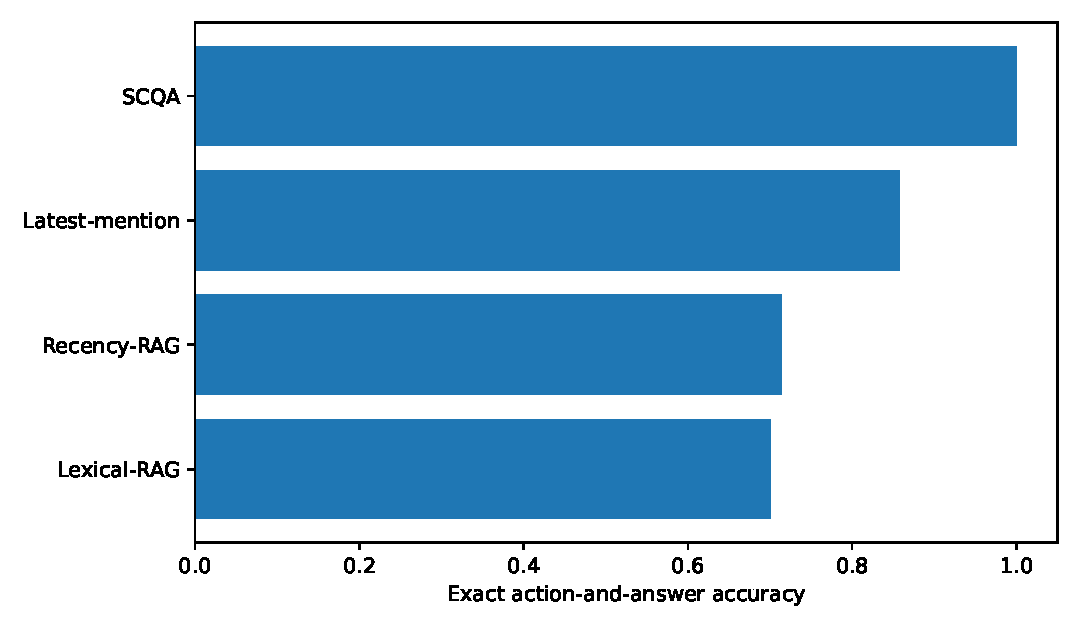
\includegraphics[width=.76\linewidth]{figures/accuracy.pdf}
\caption{Oracle-state diagnostic accuracy. The result demonstrates that the
specified invariants are executable. It does not estimate end-to-end LLM
accuracy because situation variables are supplied rather than inferred.}
\label{fig:accuracy}
\end{figure}

The category-level pattern provides the useful result. Latest mention fails on
hidden-premise items because it answers when clarification is required. Recency
ranking fails when the newest global event is not known to the queried observer.
Lexical overlap is vulnerable to weak but topically similar conflicting claims.
Thus a single aggregate ``hallucination'' label hides distinct and testable
mechanisms (Fig.~\ref{fig:category}).

\begin{figure}[t]
\centering
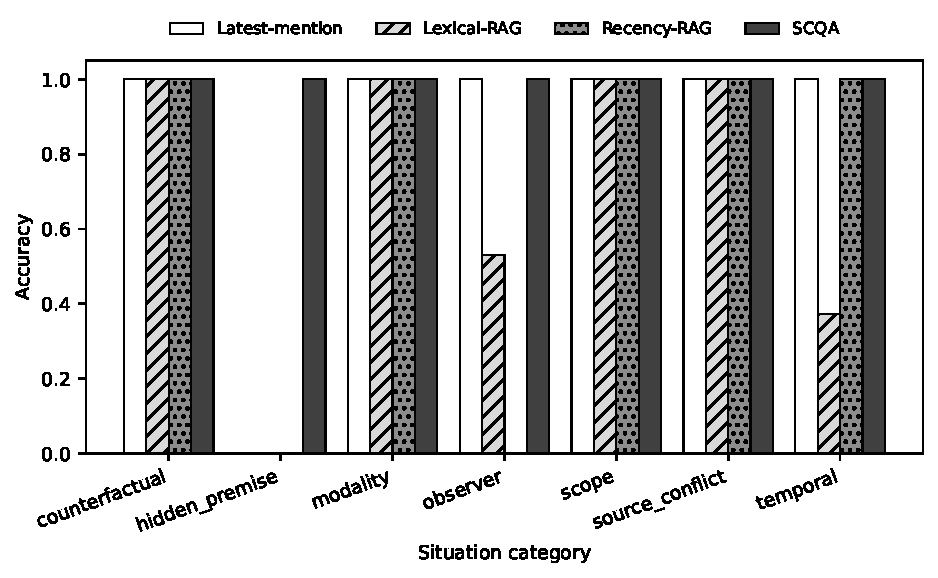
\includegraphics[width=.94\linewidth]{figures/by_category.pdf}
\caption{Accuracy by diagnostic category. Each category isolates one
applicability variable, enabling mechanism-level failure localization.}
\label{fig:category}
\end{figure}

\subsection*{Component ablations produce matched failure signatures}

Removing temporal validity, source status, modality, scope, observer knowledge,
world identity or missing-variable detection selectively damages the matching
category (Fig.~\ref{fig:ablation}). This causal alignment is the main empirical
contribution of the controlled study. It shows that the implementation does not
merely benefit from a generic instruction to be cautious; behaviour changes
when the specific variable required by an item is removed. Because benchmark
and solver share the same schema, the result is best viewed as a mechanistic
unit test that future neural systems should pass under both gold and predicted
states.

\begin{figure}[t]
\centering
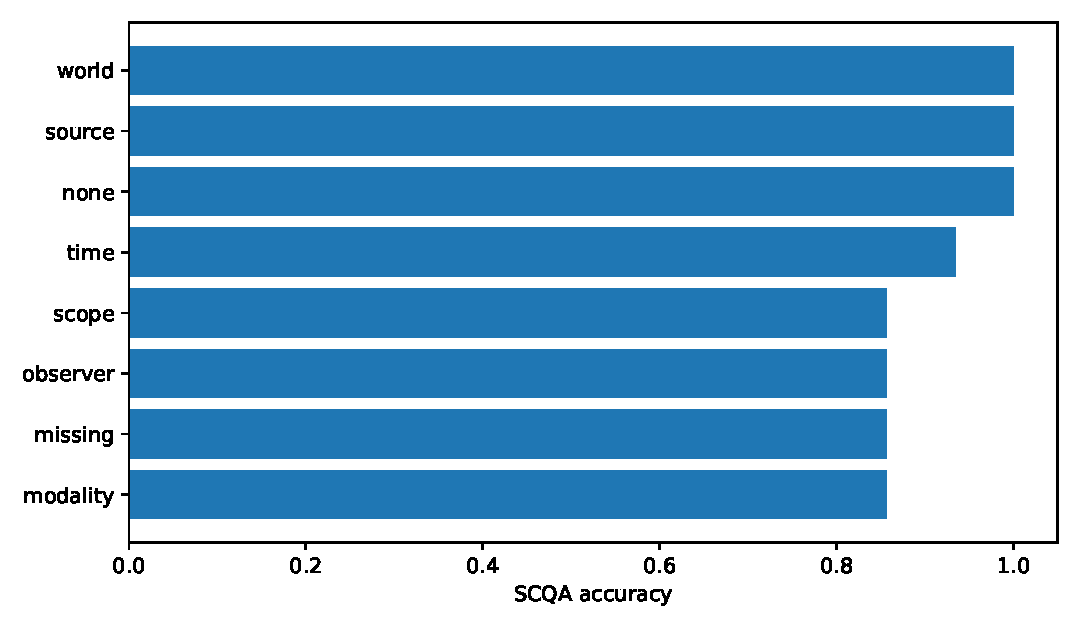
\includegraphics[width=.76\linewidth]{figures/ablations.pdf}
\caption{Oracle-state component ablations. Each removed variable recovers the
predicted category-specific failure, providing a causal software diagnostic.}
\label{fig:ablation}
\end{figure}

\subsection*{Predicted states expose a sensing bottleneck}

We removed access to the structured claim fields and reconstructed a restricted
situation state from claim text using the released deterministic sensor. Across
all 4,200 diagnostic instances, action-and-answer accuracy fell from 100.0\%
with gold states to 77.9\% with predicted states. Deliberately overwriting
source status, modality and scope in the predicted state reduced accuracy
further to 35.1\%. These are complete executions, not projected values. They
show that the oracle result is not preserved when situation sensing is
imperfect. Because the texts are generated from the same seven scenario
families and the sensor is a transparent rule baseline, these results remain
controlled diagnostics rather than evidence of natural-language or LLM
generalization.

Claim-level scoring localizes the sensor's limitations
(Table~\ref{tab:slot-sensing}). Event type reached 92.3\%, modality 100.0\%,
scope 61.5\%, actor 30.8\% and joint source/status 30.8\%. Temporal expressions
and validity intervals scored 0\% because the generated claim strings omit the
numeric times stored in the hidden schema: a system cannot reconstruct a state
variable that is neither expressed nor retrieved. Observer and world slots
reached 92.3\% and 100.0\% under repetitive generated language and are not
estimates of natural extraction. In this deterministic pipeline, 927 final
errors are attributable to sensing, zero to update/policy under gold state, and
generation is a fixed renderer.

\begin{table}[t]
\caption{Claim-level accuracy of the deterministic text sensor
($n=7{,}800$ claims per slot).}
\label{tab:slot-sensing}
\centering\scriptsize
\setlength{\tabcolsep}{3pt}%
\begin{tabular}{lrrrrrrrrr}
\toprule
Slot & Actor & Event & Time & Validity & Scope & Modality & Source & Observer & World\\
\midrule
Accuracy (\%) & 30.8 & 92.3 & 0.0 & 0.0 & 61.5 & 100.0 & 30.8 & 92.3 & 100.0\\
\bottomrule
\end{tabular}
\end{table}

\subsection*{Natural-language benchmarks establish prevalence, not SCQA efficacy}

Independent resources show that situation dependence is not confined to the
generated benchmark. SituatedQA reported that approximately 16.5\% of sampled
NQ-Open questions depended on time or place and that updated evidence did not
remove a substantial present-time performance gap~\cite{zhang2021situatedqa}.
FreshQA, PAT-Questions, TimeQA, ChronoQA and TDBench test related problems in
freshness, evolving facts and temporal validity
~\cite{vu2023freshqa,meem2024pat,chen2021timeqa,chen2025chronoqa,kim2025tdbench}.
These studies motivate the problem definition, but they are not evaluations of
SCQA and are not counted as evidence that the proposed intervention improves a
frontier model.

\subsection*{An evidence ladder separates established findings from open claims}

Table~\ref{tab:evidence-ladder} makes the claim boundary explicit. The current
study establishes that seven applicability invariants can be represented,
executed and independently ablated under oracle structured states. It supports,
but does not establish, the hypothesis that explicit situation states will
reduce analogous errors in LLMs. End-to-end efficacy requires matched
multi-model experiments on natural text, predicted-state evaluation, strong
prompt/RAG/agent baselines, clustered uncertainty estimates, human annotation
and efficiency analysis. We release the adapter, schemas and reporting protocol
for these experiments but do not substitute unexecuted predictions for results.

\begin{table}[t]
\caption{Evidence ladder and permitted interpretation.}
\label{tab:evidence-ladder}
\centering\small
\begin{tabularx}{\linewidth}{@{}>{\raggedright\arraybackslash}p{3.0cm}X>{\raggedright\arraybackslash}p{4.2cm}@{}}
\toprule
Evidence level & What is available & Permitted claim \\
\midrule
E1: formal definition & Situation schema and applicability relation & The failure class is operationally testable \\
E2: oracle unit tests & 4,200 generated instances and matched ablations & Specified invariants are executable and causally separable \\
E3: natural prevalence & Independent temporal/situated QA literature & Situation dependence occurs in natural questions \\
E4: predicted-state control & Deterministic text sensor on 4,200 generated items & Sensing errors reduce controlled end-to-end accuracy; natural-text generalization remains open \\
E5: multi-model intervention & Execution harness only; no successful model responses & Needed to claim LLM improvement and generality \\
E6: deployment / human study & Not completed & Needed for operational safety and human comparison \\
\bottomrule
\end{tabularx}
\end{table}

\ifE5ready\subsection*{Matched multi-model intervention (E5)}

The controlled results above establish that the seven applicability invariants
are executable and causally separable under oracle and predicted structured
states (E1--E4). They do not by themselves establish that supplying an explicit
situation state improves a frontier language model on natural prompts. That is
the E5 claim in the evidence ladder, and it requires model responses rather than
symbolic controls. We therefore evaluate several proprietary and open-weight
models on a stratified, evidence-complete rendering of SituationCatch-Bench
(30 items per category), holding the evidence block, decoding temperature and
output-token budget fixed and varying only the prompt condition. The primary
quantity is the situation-on-versus-off contrast within each model: the
situation-state condition minus the strongest non-situational prompt for the
same model, so any difference is attributable to explicit state rather than to
model identity, evidence or budget. Raw responses, usage, latencies and failed
calls are archived per model; the reported accuracies read directly from those
records and exclude failed calls, which are reported as $n$.

% E5 multi-model table -- PENDING.
% No real model rows were found in the summary CSV yet (only mock/empty data).
% Run:  python code/run_e5.py        (needs OPENROUTER_API_KEY with credits)
% then: python code/make_e5_table.py  to regenerate this file with real numbers.
\begin{table}[t]
\caption{E5 multi-model situation-intervention results \emph{(pending execution;
no frontier-model responses are included in this build)}. Regenerated
automatically from \texttt{paper/results/multimodel\_summary.csv} once
\texttt{code/run\_e5.py} has produced real responses.}
\label{tab:e5-multimodel}
\centering\small
\begin{tabular}{l}
\toprule
Awaiting E5 execution --- see \texttt{code/experiment\_manifest.e5.json}. \\
\bottomrule
\end{tabular}
\end{table}


We interpret a positive within-model $\Delta$ as support for the hypothesis that
explicit situation state reduces applicability errors under matched conditions,
not as evidence of deployment readiness: the rendered prompts still derive from
the seven generated scenario families, so natural-text and distributional
generalization (E5 splits and E6) remain open. The frozen study manifest,
provider gateway, model snapshots and cost accounting are recorded in
\texttt{code/experiment\_manifest.e5.json}, and the run is reproduced by a single
command (\texttt{python code/run\_e5.py}).
\fi   % E5 multi-model intervention (activate after code/run_e5.py)
\pdfbookmark[1]{Discussion}{bookmark-discussion}
\section*{Discussion}

The core insight is that relevance is not applicability. Retrieval can return a
well-supported statement while a system still applies it to the wrong time,
scope, epistemic state or possible world. Situation engineering turns this
failure from an informal complaint about ``missing context'' into a set of
state variables, update rules and behavioural consequences that can be tested
separately.

\subsection*{A complementary layer, not a replacement vocabulary}

Prompt, context, retrieval, memory, tool, harness, evaluation, security and
serving engineering retain distinct responsibilities. Prompts specify the task;
context and retrieval supply evidence; memory preserves observations; tools
provide capabilities; harnesses govern workflow and permissions; evaluations
measure behaviour; serving systems manage resource constraints. Situation
engineering owns the query-relative semantics of the active state and the
propagation of unresolved applicability into policy. A useful contract is
\begin{equation}
(C_t,M_t,O_t,H_t)\rightarrow(\mathcal{S}_t,U_t,P_t),
\end{equation}
where context, memory, tool observations and harness traces produce candidate
situations $\mathcal{S}_t$, unresolved variables $U_t$ and the permitted policy
$P_t$.

This contract prevents conceptual inflation. Retrieval quality should not be
renamed situation engineering, and a JSON field named ``situation'' is not
evidence of situation awareness. A system must show that state representation
causally changes behaviour in predicted cases, that state uncertainty affects
answering or action, and that failures can be assigned to sensing, update,
validation, policy or generation.

\subsection*{Implications for hallucination and agent evaluation}

A generated claim can be textually entailed by a document yet wrong for the
query. Evaluation should therefore record both support and applicability. In
free-form generation, claims should be linked to the situation state and
provenance on which they depend. In agents, tools should expose preconditions,
state transitions and failure semantics rather than only free-text outputs;
harnesses should block consequential actions while answer-critical state is
unresolved. Evaluation engineering becomes the sensor layer that checks each
transition and not merely the final answer.

The response policy is also part of correctness. Clarification and abstention
are not failures when the situation is under-specified. Conversely, excessive
clarification is costly and can make systems unusable. Future evaluations should
therefore report answer accuracy, clarification utility, unnecessary-question
rate, abstention precision, selective risk, coverage, latency, token use and
monetary cost. These measures make explicit the trade-off between semantic
verification and serving efficiency.

\subsection*{What is established and what remains to be tested}

This study demonstrates a formal error class, an interoperable state schema and
category-specific causal effects of matched state ablations. It also shows that
performance degrades sharply when state must be recovered from partially
observable text. Together, these results identify situation sensing as a
separate engineering and evaluation target rather than treating every failure
as retrieval or generation error.

The controlled design cannot decide whether the full interface improves a
contemporary language model beyond a matched structured prompt or temporal RAG.
That comparison is the confirmatory submission gate for the general LLM claim:
same model, evidence and computation budget; independently authored natural
questions; direct, structured, temporal-retrieval, verification-agent and
situation conditions; and paired, scenario-clustered inference. The released
protocol makes this contrast executable, while the present results make no
claim from incomplete pilot calls. The SE0--SE4 maturity model and longer
research programme are provided in Supplementary Information.

\subsection*{Limitations and risks}

The diagnostic data are generated from a schema shared with the solver, so
benchmark-solver circularity is intentional and limits external validity. The
item count overstates statistical independence because examples share template
families. The baselines are software controls, not state-of-the-art LLM
systems. Confidence values are rule-derived and do not constitute neural
calibration. No human participants, multilingual evaluation, multimodal sensing or
deployed-agent study was completed. A small Gemini API pilot verified the
execution path but ended at unequal category coverage when free-tier quota was
exhausted; it is excluded from scientific results. These limitations
are not resolved by additional prose and require new experiments.

Explicit state can also create new attack surfaces. An adversary may manipulate
timestamps, source authority, identity, scope or world labels. A centralized
state representation may expose sensitive user information or create false
confidence in a flawed schema. Situation-engineered systems therefore require
provenance, access control, privacy-preserving memory, conflict visibility and
independent evaluation. ``Explicit'' must not be confused with ``correct''.

\subsection*{Conclusion}

Situation engineering provides a bounded and testable interface between
retrieval, state estimation and response policy. The controlled experiments
demonstrate that applicability variables have distinct behavioural consequences
and that imperfect sensing can erase the advantage of correct update rules.
Establishing broad utility now requires the pre-specified natural-text,
multi-model comparison against equally resourced structured prompting,
temporal retrieval and agent verification.


%% ---- Methods (Nature: starred section, not counted in word limit) ----
\pdfbookmark[1]{Methods}{bookmark-methods}
\section*{Methods}

\subsection*{Problem formulation}

An item consists of a query $q$, evidence claims $E$, a query time and, where
relevant, an observer or possible-world identifier. A claim may be supported in
isolation but inapplicable to the query. We define
\begin{equation}
\mathrm{Apply}(e,q,S)\in\{\mathrm{valid},\mathrm{invalid},\mathrm{unresolved}\},
\end{equation}
where $S$ is the active situation state. The system first constructs or receives
$S$, then updates competing claims and selects an action from answering,
retrieval, clarification, abstention or task-specific action.

The end-to-end system is decomposed as
\begin{equation}
(q,E)\xrightarrow{f_{sense}}\hat S\xrightarrow{f_{update}}\hat S'
\xrightarrow{\pi}a\xrightarrow{g}y.
\end{equation}
This decomposition supports stage-specific evaluation. The gold-state condition
supplies $S$ directly and evaluates $f_{update}$, $\pi$ and the deterministic
answer renderer. A predicted-state condition applies a text-only deterministic
sensor before the same update and policy stages. It evaluates composition on
generated claim language, but not $f_{sense}$ on unrestricted natural language.

\subsection*{Situation schema}

The schema contains actors and entities; events and state transitions; valid
and observation time; scope; modality and source status; observer-specific
knowledge; possible-world identity; provenance; and unresolved answer-critical
variables. Update rules include temporal supersession, cancellation,
source-authority preference where specified, scope containment, observer
visibility and world separation. Unresolved variables are preserved rather than
converted into a guessed binary state.

\subsection*{SituationCatch-Bench generation}

The deterministic generator creates 600 instances for each of seven categories
using seeded lexical variation and shuffled claim order. Each item includes the
question, claims, structured situation fields, gold action, gold answer aliases
and category. The categories and gold semantics are documented in the bundled
datasheet. Generation and evaluation are intentionally co-designed: the
benchmark is a conformance suite for explicit semantics, analogous to unit tests
for a software protocol, rather than an independent estimate of natural-language
performance.

Future benchmark versions should use separate authors for data construction and
system development, clustered scenario families, hidden generators, natural and
semi-synthetic sources, adjudicated annotations, compositional splits and
adversarial state manipulations. Recommended natural-data fields and annotation
instructions are supplied in the Supplementary Information.

\subsection*{Reference implementation}

SCQA is a deterministic Python reference implementation with no trained
parameters. It parses the supplied structured fields, performs category-specific
state updates and selects a permitted response. The three software-control
baselines select claims using lexical overlap, recency or latest mention and do
not maintain the complete situation state. These controls test whether the
specified state variables are necessary for the generated invariants; they are
not intended to represent competitive LLM, RAG or agent baselines.

\subsection*{Predicted- and corrupted-state evaluation}

The predicted-state sensor receives only claim text and infers event type,
actor, temporal expression, modality, source status and world or scope using
documented deterministic patterns; it cannot copy hidden gold slots. The
downstream engine is unchanged. In a pre-specified corruption condition,
predicted source status is replaced by a generic reported source, modality is
forced to confirmed and scope is forced to global. All three conditions contain
the same 4,200 identifiers and are scored by exact action and answer. Item-level
and aggregate outputs are released in
\texttt{results/state\_conditions.csv} and
\texttt{results/state\_conditions\_summary.csv}.
The sensor is additionally scored claim by claim for actor, event, temporal
expression, validity interval, scope, modality, joint source/status,
observer-knowledge and world slots. Because claim order is preserved, this
comparison does not require learned alignment. The resulting files are
\texttt{results/predicted\_state\_slots.csv} and its aggregate summary.

\subsection*{Metrics and analysis}

The primary diagnostic measure is exact action-and-answer accuracy. For items
requiring clarification, correctness requires selecting clarification rather
than providing the latent answer. Category-level accuracy and matched component
ablations localize failure mechanisms. Because instances share template
families, item-level confidence intervals and $P$ values are not used as primary
scientific evidence in the revised manuscript. The released scripts retain
item-level summaries for regression testing, but future natural-language studies
should use scenario- or template-clustered bootstrap intervals, paired tests,
multiple-comparison control and pre-specified primary outcomes.

Rule-derived confidence values from the original implementation are not treated
as neural calibration. End-to-end work should report Brier score, expected
calibration error, selective risk, risk--coverage area, clarification utility
and abstention precision/recall using model- or state-derived probabilities.

\subsection*{Ablation design}

Seven ablations independently remove temporal validity, source status, modality,
scope, observer knowledge, world identity or missing-variable detection. Each
ablation is applied to all items, and its expected effect is specified before
execution. The purpose is to test causal alignment between representation and
failure category, not to estimate an average treatment effect in natural text.

\subsection*{Protocol for end-to-end multi-model evaluation}

A confirmatory study should compare at least the following matched conditions:
direct prompting; chain-of-thought or structured prompting; date-aware context;
standard RAG; temporal or event-aware RAG; reflection or verification agent; and
Situation Engineering. The generation model, evidence set, retrieval corpus,
maximum context, output budget and sampling parameters should be held constant
where the design permits. At least three proprietary and three open-weight model
families should be evaluated using immutable model identifiers.

The primary intervention contrast must be
\emph{same model + same evidence + same computation budget} with versus without
the explicit situation layer. A factorial analysis should independently vary
prompt, context/retrieval, harness and situation state. Competitive conditions
should include long-context prompting, few-shot structured reasoning,
self-consistency, self-refinement, Self-RAG, graph or temporal retrieval,
dialogue/belief-state tracking, clarification and calibrated abstention.

For each call, researchers should archive the prompt, evidence, raw response,
normalized answer, action decision, model identifier, provider, execution date,
latency, token use, monetary cost, errors and retries. Evaluation must report
gold-state, predicted-state and deliberately corrupted-state conditions. The
predicted-state condition should score entity/event extraction, temporal
relations, validity intervals, scope, modality, source status, observer
knowledge, possible-world identity and final answer. This enables error
attribution to sensing, updating, policy or generation.

The bundled \texttt{code/run\_multimodel\_eval.py} provides provider adapters and
refuses to create placeholder outputs when credentials are absent. No
frontier-model performance values are reported because such calls were not
executed in the study environment. The script is an executable protocol, not a
completed experiment.

\subsection*{Generalization and efficiency protocol}

External evaluation should pre-register held-out scenario families and test
unseen templates, longer event chains, nested scopes, conflicting authoritative
sources, multiple observers, multilingual questions and adversarial stale
evidence. Splits must occur at scenario or generator-grammar level rather than
over lexical variants. Uncertainty intervals should use scenario-clustered
resampling. Each condition must report latency, input and output tokens,
retrieval and tool calls, retries, monetary cost and clarification overhead.
Accuracy gains without matched resource reporting cannot identify the effect of
the situation layer.

\subsection*{Human and deployment evaluation}

Human evaluation should use at least three independent annotators per natural
item, blinded to method, with a documented adjudication procedure. Recommended
outcomes include state-slot agreement, answer correctness, appropriateness of
clarification or abstention, unnecessary clarification and perceived
justification quality. Studies involving participants should report ethics
approval or exemption, consent, compensation and privacy handling.

The released annotation program generates separately shuffled, blinded packets
for three or more annotators. It requires complete independent labels before
computing Fleiss' $\kappa$ and unanimous agreement for action, answer and state
slots; incomplete packets terminate with an error. Disagreements are adjudicated
only after independent files are frozen. No human agreement value is reported
because independent human annotations were not collected.

Deployment studies should additionally measure state drift, invalidation
latency, recovery after contradictory observations, action-precondition
violations, security attacks on state metadata, throughput, tail latency,
energy, token use and cost. The state and provenance required to audit a
consequential decision should be retained subject to privacy and access-control
requirements.

\subsection*{Reproducibility and reporting protocol}

The package contains the generator, generated benchmark, reference
implementation, predictions, figures, datasheet and exact commands. To make
future systems comparable, authors should report: (1) the situation schema;
(2) which variables are supplied, retrieved or inferred; (3) update and conflict
semantics; (4) response and action policies; (5) provenance and observability;
(6) stage-specific errors; (7) prompt, context, retrieval, memory, tool and
harness configurations; and (8) resource costs. A machine-readable experiment
manifest is recommended.

\subsection*{Ethics and use of generative AI}

The controlled benchmark contains no personal records or human participants.
Generative AI assisted drafting and software development. The author inspected
the code, generated outputs, calculations and references and remains responsible
for the manuscript. No empirical values were fabricated to represent unexecuted
model calls or human studies.


%% ---- Data availability (Nature Portfolio: standalone statement) ----
\section*{Data availability}
SituationCatch-Bench v0.1 is included in the public source repository at
\url{https://github.com/leemgs/sage} and in the submission package as
\texttt{data/situationcatch\_bench.jsonl}, together with its deterministic
generator, datasheet and item-level outputs. This package is sufficient to
reproduce the controlled results. The exact reviewed version is identified by
the Git commit attached to the submission. An immutable archival release, an
institutionally approved licence and DOI remain required before acceptance; no
placeholder DOI is represented as an existing deposit.

%% ---- Code availability (Nature Portfolio: standalone statement) ----
\section*{Code availability}
The complete executable implementation is included under \texttt{code/}.
Running \texttt{PYTHONPATH=code python code/run\_experiments.py}
regenerates gold-, predicted- and corrupted-state outputs without network
access or proprietary dependencies. The multi-model adapter records raw
responses and errors and never creates synthetic API results. The annotation
program requires three complete independent packets before reporting agreement.
Source and item-level outputs are also available at
\url{https://github.com/leemgs/sage}. The repository README records exact
commands; \texttt{SHA256SUMS.txt} records packaged artefact checksums. A public
immutable release and archival DOI remain pre-acceptance requirements.

%% ---- Author Contributions ---------------------------------
\section*{Author Contributions}
G.L.: Conceptualization, Formal analysis, Investigation, Methodology,
Software, Validation, Visualization, Writing -- original draft,
Writing -- review \& editing.

%% ---- Competing Interests ----------------------------------
\section*{Competing Interests}
The author declares no competing interests.

%% ---- Acknowledgements -------------------------------------
\section*{Acknowledgements}
The author received no specific funding for this work.


%% ---- References -------------------------------------------
\begin{thebibliography}{26}
% REVIEW COPY: URLs are printed to support pre-submission reading of each
% reference. For the journal-submission version set \RefURLsfalse in main.tex
% (the \refurl{...} fields below are then suppressed automatically).
\bibitem{lewis2020rag} Lewis, P. et al. Retrieval-augmented generation for knowledge-intensive NLP tasks. \emph{Adv. Neural Inf. Process. Syst.} \textbf{33}, 9459--9474 (2020).\refurl{https://arxiv.org/abs/2005.11401}
\bibitem{asai2024selfrag} Asai, A., Wu, Z., Wang, Y., Sil, A. \& Hajishirzi, H. Self-RAG: learning to retrieve, generate, and critique through self-reflection. In \emph{Proc. International Conference on Learning Representations} (2024).\refurl{https://openreview.net/forum?id=hSyW5go0v8}
\bibitem{yao2023react} Yao, S. et al. ReAct: synergizing reasoning and acting in language models. In \emph{Proc. International Conference on Learning Representations} (2023).\refurl{https://openreview.net/forum?id=WE_vluYUL-X}
\bibitem{schick2023toolformer} Schick, T. et al. Toolformer: language models can teach themselves to use tools. \emph{Adv. Neural Inf. Process. Syst.} \textbf{36} (2023).\refurl{https://proceedings.neurips.cc/paper_files/paper/2023/hash/d842425e4bf79ba039352da0f658a906-Abstract-Conference.html}
\bibitem{zhang2021situatedqa} Zhang, M. J. Q. \& Choi, E. SituatedQA: incorporating extra-linguistic contexts into QA. In \emph{Proc. EMNLP}, 7371--7387 (2021).\refurl{https://aclanthology.org/2021.emnlp-main.586/}
\bibitem{allen1983interval} Allen, J. F. Maintaining knowledge about temporal intervals. \emph{Commun. ACM} \textbf{26}, 832--843 (1983).\refurl{https://doi.org/10.1145/182.358434}
\bibitem{mei2025context} Mei, L. et al. A survey of context engineering for large language models. \emph{Preprint at} arXiv (2025).\refurl{https://arxiv.org/abs/2507.13334}
\bibitem{zhong2026harness} Zhong, H. \& Zhu, S. AI harness engineering: a runtime substrate for foundation-model software agents. \emph{Preprint at} arXiv (2026).\refurl{https://arxiv.org/abs/2605.13357}
\bibitem{lin2026ahe} Lin, J. et al. Agentic harness engineering: observability-driven automatic evolution of coding-agent harnesses. \emph{Preprint at} arXiv (2026).\refurl{https://arxiv.org/abs/2604.25850}
\bibitem{barwise1983situations} Barwise, J. \& Perry, J. \emph{Situations and Attitudes} (MIT Press, 1983).\refurl{https://mitpress.mit.edu/9780262521093/situations-and-attitudes/}
\bibitem{vu2023freshqa} Vu, T. et al. FreshLLMs: refreshing large language models with search engine augmentation. \emph{Preprint at} arXiv (2023).\refurl{https://arxiv.org/abs/2310.03214}
\bibitem{meem2024pat} Meem, J. et al. PAT-Questions: a self-updating benchmark for present-anchored temporal question answering. In \emph{Findings of ACL} (2024).\refurl{https://aclanthology.org/2024.findings-acl.777/}
\bibitem{chen2021timeqa} Chen, W., Wang, X., Wang, W. Y. \& Chen, W. A dataset for answering time-sensitive questions. In \emph{NeurIPS Datasets and Benchmarks} (2021).\refurl{https://openreview.net/forum?id=Mn1lWz3F4x}
\bibitem{chen2025chronoqa} Chen, Z. et al. ChronoQA: a question answering dataset for temporal-sensitive retrieval-augmented generation. \emph{Sci. Data} (2025).\refurl{https://www.nature.com/articles/s41597-025-05757-2}
\bibitem{kim2025tdbench} Kim, S., Wang, J., Xie, X. \& Whang, S. E. Harnessing temporal databases for systematic evaluation of factual time-sensitive question answering in large language models. \emph{Preprint at} arXiv (2025).\refurl{https://arxiv.org/abs/2508.02045}
\bibitem{vanbenthem1996dynamic} van Benthem, J. Dynamic logic for belief revision. \emph{J. Appl. Non-Classical Logics} \textbf{6}, 129--155 (1996).\refurl{https://doi.org/10.1080/11663081.1996.10510843}
\bibitem{stalnaker2002common} Stalnaker, R. Common ground. \emph{Linguist. Philos.} \textbf{25}, 701--721 (2002).\refurl{https://doi.org/10.1023/A:1020867916902}
\bibitem{alchourron1985logic} Alchourr\'{o}n, C. E., G\"ardenfors, P. \& Makinson, D. On the logic of theory change: partial meet contraction and revision functions. \emph{J. Symb. Logic} \textbf{50}, 510--530 (1985).\refurl{https://doi.org/10.2307/2274239}
\bibitem{doyle1979truth} Doyle, J. A truth maintenance system. \emph{Artif. Intell.} \textbf{12}, 231--272 (1979).\refurl{https://doi.org/10.1016/0004-3702(79)90008-0}
\bibitem{kaelbling1998pomdp} Kaelbling, L. P., Littman, M. L. \& Cassandra, A. R. Planning and acting in partially observable stochastic domains. \emph{Artif. Intell.} \textbf{101}, 99--134 (1998).\refurl{https://doi.org/10.1016/S0004-3702(98)00023-X}
\bibitem{henderson2014second} Henderson, M., Thomson, B. \& Williams, J. D. The second dialog state tracking challenge. In \emph{Proc. SIGDIAL}, 263--272 (2014).\refurl{https://aclanthology.org/W14-4337/}
\bibitem{snodgrass1992temporal} Snodgrass, R. T. Temporal databases. In \emph{Theories and Methods of Spatio-Temporal Reasoning in Geographic Space}, 22--64 (Springer, 1992).\refurl{https://doi.org/10.1007/3-540-55966-3_3}
\bibitem{kwon2023pagedattention} Kwon, W. et al. Efficient memory management for large language model serving with PagedAttention. In \emph{Proc. ACM SOSP}, 611--626 (2023).\refurl{https://arxiv.org/abs/2309.06180}
\bibitem{mccarthy1969problems} McCarthy, J. \& Hayes, P. J. Some philosophical problems from the standpoint of artificial intelligence. In \emph{Machine Intelligence 4}, 463--502 (1969).\refurl{https://www-formal.stanford.edu/jmc/mcchay69.pdf}
\bibitem{kowalski1986event} Kowalski, R. \& Sergot, M. A logic-based calculus of events. \emph{New Gener. Comput.} \textbf{4}, 67--95 (1986).\refurl{https://doi.org/10.1007/BF03037383}
\bibitem{reiter2001knowledge} Reiter, R. \emph{Knowledge in Action: Logical Foundations for Specifying and Implementing Dynamical Systems} (MIT Press, 2001).\refurl{https://mitpress.mit.edu/9780262681495/knowledge-in-action/}
\end{thebibliography}


%% ---- Supplementary Information --------------------------------
%% NMI: submitted as a SEPARATE file — see supplementary.tex
%% (builds supplementary.pdf; Supplementary Notes 1–5, Tables 1–11).

\end{document}
